\documentclass[]{IEEEtran}
%\IEEEoverridecommandlockouts
% The preceding line is only needed to identify funding in the first footnote. If that is unneeded, please comment it out.
\usepackage{cite}

% Your packages go here
\usepackage[utf8]{inputenc}
\usepackage{romannum}
\usepackage{graphicx}
\usepackage{caption,subcaption}
\usepackage{listings}
\usepackage{color}
\usepackage{url}
\usepackage{amsmath}
\usepackage{nccmath}
\usepackage{mathtools}

\DeclarePairedDelimiter{\norm}{\lVert}{\rVert}

\definecolor{dkgreen}{rgb}{0,0.6,0}
\definecolor{gray}{rgb}{0.5,0.5,0.5}
\definecolor{mauve}{rgb}{0.58,0,0.82}

\lstset{frame=tb,
  language=python,
  aboveskip=3mm,
  belowskip=3mm,
  showstringspaces=false,
  columns=flexible,
  basicstyle={\small\ttfamily},
  numbers=none,
  numberstyle=\tiny\color{gray},
  keywordstyle=\color{blue},
  commentstyle=\color{dkgreen},
  stringstyle=\color{mauve},
  breaklines=true,
  breakatwhitespace=true,
  tabsize=3,
  literate={á}{{\'a}}1
           {ç}{{\c{c}}}1
           {ü}{{\"u}}1
           {é}{{\'e}}1
}

\def\BibTeX{{\rm B\kern-.05em{\sc i\kern-.025em b}\kern-.08em
    T\kern-.1667em\lower.7ex\hbox{E}\kern-.125emX}}

\markboth{MC949/MO446 Computer Vision - HW2}{}

\begin{document}
  \title{Video Augmented Reality}
  \author{Darley Barreto, Edgar Tanaka, Tiago Barros
    \thanks{228120, 023577, 093125}
  }
  \maketitle

  \begin{abstract}
    In this work, we implemented a pipeline capable of reading a video and producing another video with augmented reality, $e.g$ placing an image inside a rectangular surface in the video. Our pipeline finds interest points, that is, feature descriptors, then matches these descriptors in different video frames with a $Kd$-tree and uses RANdom SAmple Consensus (RANSAC) to find the best affine transformation capable of mapping data between frames. The final video produced contained an image that was pasted on top of a blue paper in rectangular shape.
  \end{abstract}

  \section{Introduction}
    An augmented reality task is the one that creates a view of a real scene that visually incorporates into the scene computer-generated images of virtual objects or images of real life objects. One motivation for augmenting reality in this way is to enhance the performance of real world tasks. In this work, we intend to place a target image (smaller image of a dog) inside a target frame (a blue rectangle detected). This transformation is applied in several video frame images so that combined they produce the augmented reality effect.

    We begin by detecting the interest points (keypoints) using our own implementation of Scale-Invariant Feature Transform (SIFT)~\cite{iccv99}. After the detection, we perform the matching using $Kd$-tree and filtering the distances given a radius $r$.

    Once we compute the matched keypoints, we used a naive version of RANSAC\cite{ransac} to find the best affine transformation for these matched keypoints. At the end, we apply this affine transformation on the target image and paste it into the video frame. Throughout this work, we show examples of each task results and we discuss them. Finally we show the result of our pipeline.

  \section{Interest points and Feature descriptors}
  To detect the keypoints, in our case the four corners of the blue paper, we implemented a version of the SIFT. SIFT is an algorithm published by David Lowe in 1999 and patented by the University of British Columbia in Canada. It detects keypoints in images and describes its features. Being invariant to image scaling, translation, and rotation, and partially invariant to illumination changes and affine or 3D projection, SIFT is often used to match different images from the same scene or images from the same camera taken in $\Delta t$ time, as is the case of this project. The basic algorithm works as follows: SIFT builds a scale space, which is basically a set of the input image in different sizes and scales of blurring. This is used to simulate viewing a scene from different amounts of distance, and, in doing so, obtain a scale-invariant procedure. When we blur an image, it loses some of its high-frequency elements, i.e. details. So, depending on the feature we want to focus on, we can look at an image with a low-scale blurring (closer to the image - details are more visible) or look at the image with a high-scale blurring (farther from the image - details are less visible). An example of scale space can be seen in the figure~\ref{fig:scale_space}.

\begin{figure}[h]
  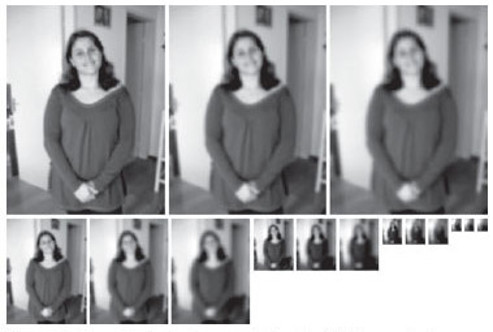
\includegraphics[width=\linewidth]{./figures/sift/scale_space.jpg}
  \caption{Example of a scale space.}
  \label{fig:scale_space}
\end{figure}

  With the scale space built, the algorithm computes differences of Gaussians (a computationally cheaper substitute for Laplacian) for each pair of horizontally adjacent pictures in the figure 1 that has the same size. Every extremum (point of maximum or minimum) of a difference of Gaussians is a candidate of approximation of keypoint. These approximations are refined using Taylor expansion. A candidate is then removed if it does not have enough contrast or if it is an edge. The remaining ones are actual keypoints.

  To assign an orientation to a keypoint, we collect gradient magnitudes and directions around it, then we assign the most prominent orientation (or orientations) in that region. The final step is to compute the descriptors, which is done by considering a 16x16 window around a keypoint, then splitting that window into 16 4x4 windows and calculating the gradient orientations using 8-bins histograms.

\begin{figure}[h]
  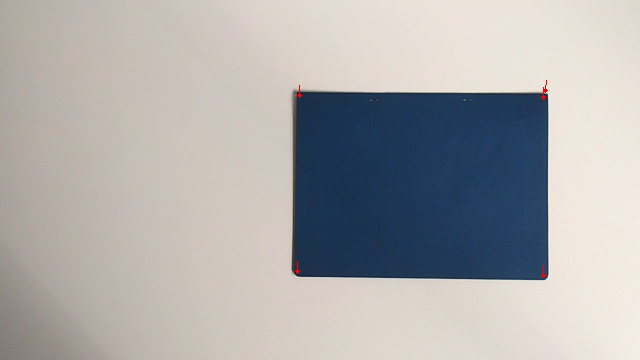
\includegraphics[width=\linewidth]{./figures/sift/four_corners.png}
  \caption{Example of feature detection: the SIFT algorithm detected the four corners of the blue rectangle.}
  \label{fig:four_corners}
\end{figure}

  An example of feature detection using the implemented algorithm and one video frame can be seen in figure~\ref{fig:four_corners}.

  To work, SIFT needs some parameters. In our implementation, they are: SIGMA1, SIGMA2, PIXEL THRESHOLD, CURVATURE THRESHOLD, FEATURE VECTOR THRESHOLD, number of octaves, and number of scales. SIGMA1 is the standard deviation of the first Gaussian blur applied to the input image. It is the $\sigma$ in the Gaussian function:

  \[G(x) = \frac{1}{\sqrt{2 \pi} \sigma} \exp(\frac{-x^2}{2 \sigma^2})\]

  According to Lowe~\cite{ijcv04}, using at least $\sigma = 0.5$, we prevent significant aliasing. This is applied just before doubling the size of the image, which, again according to Lowe, increases the number of stable keypoints by almost a factor of 4~\cite{ijcv04}. After doubling the image and before creating the first octave of scale space, we need some additional smoothing. SIGMA2 is the standard deviation of this second Gaussian blur. We chose SIGMA1~$= 0.7$ and SIGMA2~$= 1.2$ by systematically experimenting with these values. Our criteria was that the algorithm detected the four corners of the blue rectangle on the maximum number of frames as possible, while minimizing the total number of detected keypoints, so that we focus on the real points of interest.

  PIXEL THRESHOLD is the minimum value (contrast) of a keypoint candidate to not be removed from the pool of candidates by the contrast criterion. We use PIXEL THRESHOLD~$= 0.03$, which was chosen as to keep the final keypoints to a minimum, while not discarding the corners.

  CURVATURE THRESHOLD is used to calculate the following threshold:

  \[maxCurvature = \frac{(CURVATURE\_THRESHOLD + 1) ^ 2} {CURVATURE\_THRESHOLD}\]

  Then, the Hessian matrix $H$ is computed and the curvature ratio is obtained through its trace $tr(H)$ and determinant $det(H)$:

  \[H =
  \begin{bmatrix}
     D_{xx} & D_{xy} \\
     D_{xy} & D_{yy}
  \end{bmatrix}\]

  \[tr(H) = D_{xx} + D_{yy}\]

  \[det(H) = D_{xx} D_{yy} - (D_{xy}) ^ 2\]

  \[curvatureRatio = \frac{tr(H) ^ 2}{det(H)}\]

  If $det(H) < 0$ or $curvatureRatio > maxCurvature$, the keypoint is removed from the pool of candidates. This is used to remove keypoint candidates on edges. We chose CURVATURE THRESHOLD~$= 12.0$. We started with the value of $10.0$, used by Lowe~\cite{ijcv04} and tweaked it to minimize the keypoints detected on edges in our experiments.

  FEATURE VECTOR THRESHOLD is used to reduce the influence of large gradient magnitudes in the feature vector caused by non-linear illumination changes. After the feature vector is computed, it is normalized to unit length, then we threshold every value in the unit vector that is greater than FEATURE VECTOR THRESHOLD. Then we normalize the feature vector again to unit length. In our implementation, we use FEATURE VECTOR THRESHOLD~$= 0.2$, which is the same value determined experimentally by Lowe~\cite{ijcv04}.

  The number of octaves and the number of scales define the size of the scale space. After exhaustively experimenting with these parameters, we settled on $2$ octaves and $1$ scale (the algorithm uses this number $+ 3$), which produced decent results and did not slow down too much the execution.

  \section{Match Hypothesis}
  In this section, we discuss the feature matching method and how we are using it. In order to perform the matching, we use the method of $Kd$-tree\cite{kd_tree} to search similarity of feature descriptors.
  The $Kd$-tree is a binary tree in which every node is a $K$-dimensional point. Points to the left of the hyperplane represent the left sub-tree of that node and the points to the right of the hyperplane represents the right sub-tree\cite{sift_kdtree}. Figure \ref{fig:kdtree} show a visual illustration of a simple $Kd$-tree.

\begin{figure*}[tb]
  \centering
  \begin{tabular}{c c}
  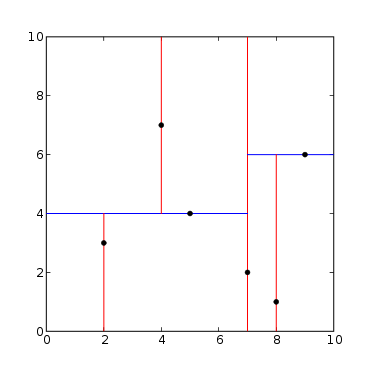
\includegraphics[width=0.23\linewidth]{./figures/kdtree/kdtree_2d.png} &
  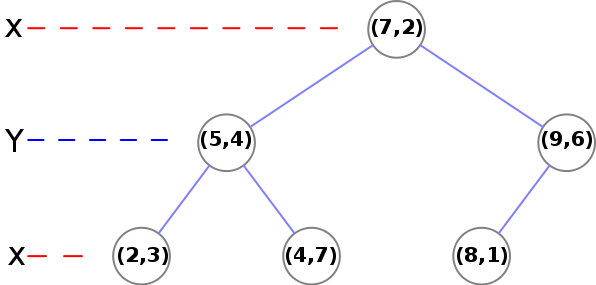
\includegraphics[width=0.4\linewidth]{./figures/kdtree/kdtree.png}\\
  a.~ $Kd$-tree decomposition for the point set & b.~ The resulting $Kd$-tree. From Wikipedia \cite{wikipedia_kd1d}.\\
  (2,3), (5,4), (9,6), (4,7), (8,1), (7,2). & \\
From Wikipedia \cite{wikipedia_kd2d}.
  \end{tabular}
  \caption{$Kd$-tree toy example.}
  \label{fig:kdtree}
\end{figure*}

  The hyperplane direction is chosen in the following way: every node split to sub-trees is associated with one of the k-dimensions, such that the hyperplane is perpendicular to that dimension vector. So, for example, if for a particular split the ``x'' axis is chosen, all points in the subtree with a smaller ``x'' value than the node will appear in the left subtree and all points with larger ``x'' value will be in the right subtree \cite{kd_tree}.
  Since there are many possible ways to choose axis-aligned splitting planes, there are many different ways to construct k-d trees. The canonical method of $Kd$-tree construction has the following constraints\cite{comp_geo}:
    \begin{enumerate}
      \item As one moves down the tree, one cycles through the axes used to select the splitting planes. (For example, the root would have an x-aligned plane, the root's children would both have y-aligned planes, the root's grandchildren would all have z-aligned planes, the next level would have an x-aligned plane, and so on.)
      \item Points are inserted by selecting the median of the points being put into the subtree, with respect to their coordinates in the axis being used to create the splitting plane. (Note the assumption that we feed the entire set of points into the algorithm up-front.)
    \end{enumerate}
  This method leads to a balanced $Kd$-tree, in which each leaf node is about the same distance from the root. However, balanced trees are not necessarily optimal for all applications. Their proven average running times in an $n$ size input are: insertion, $O(\log n)$; deletion of the root, $O(n (k-1)/k)$; deletion of a random node, $O(\log n)$; and optimization (guarantees logarithmic performance of searches), $O(n \log n)$. Search algorithms are given for partial match queries with $t$ keys specified, proven maximum running time of $O(n (k-t)/k)$, and for $k$ nearest neighbors queries empirically observed average running time of $O(k \log n)$\cite{kd_tree}.

  To find the $k$ nearest neighbors, we begin at the root of the tree. Our point must lie either on the left or right partition, but not both. That is, we can eliminate an entire part of the $Kd$-tree by determining which point is closer by a metric distance like Euclidean. Hence, we can eliminate the partition and continue recursively until the bottom of the tree. It is possible that you could finish earlier, if the current root is closer to the query point than either of its children. If so, save that as the current best and continue down the tree. In order to find the $k$ nearest neighbors, we simply repeat this operation $k$ times.

  So we create a $Kd$-tree for the set of image descriptors in one image (video frame) and perform a query with the descriptors from the immediate next frame. Thus we begin with the first frame sampled from the video, then build one $Kd$-tree, after, query with the descriptors from the second frame, then create another $Kd$-tree for the second frame, query with the third frame and so on. Each query gives us closest neighbor of a descriptor, then we need to check if this neighbor is closer to that descriptor in a radius $r$ set by the user. If so, we get the key point related to that descriptor and return as a possible match. Finally, for each pair of frames, we have the possible matches between them.

  The matching approach is based on the distance measure between the descriptors after a $Kd$-tree search. If the Euclidean distance of descriptors among the initial matches is too small then $Kd$-tree search fails. Note that there are points which are correctly detected but are rejected by the distance measure.  However, these points matched by using a more distinctive descriptor or by applying semi-local constraints\cite{sift_kdtree}.

  In Figure \ref{fig:matches} we apply the $Kd$-tree based feature matching (a) in two different frames and compare with OpenCV's implementation of Fast Approximate Nearest Neighbor Search (FLANN)\cite{flann} (b) in the same images. In this test we extract the distances and keypoints using OpenCV's SIFT function. Although one keypoint in the right frame is matched with more than one in the left frame, our implementation and OpenCV's have three keypoints in common. As we believe OpenCV has a good implementation, we also believe our results for these images are good ones.

  Once we have the possible matches between two images (video frames), we want to learn the transformation between our two images and perform the model verification. We can do this by minimizing the least squares error for the parameters of the affine transformation relating the model to the image. We use the RANSAC\cite{ransac} method in order to find the model which best fits our data. At least 3 matches are needed to provide a solution. We can write this linear system as
  \begin{equation} \label{eq:linear_sys}
  \mathbf{XA} \approx \mathbf{Y}
  \end{equation}
  where $\mathbf{X}$ is a known $m$-by-$n$ matrix (usually with $m > n$), $\mathbf{A}$ is an unknown $n$-dimensional parameter vector, and $\mathbf{Y}$ is a known $m$-dimensional measurement vector. Therefore, the minimizing vector $\mathbf{A}$  is a solution of the normal equation
  $$
  \mathbf{X}^T\mathbf{X}\mathbf{A} = \mathbf{X}^T\mathbf{Y}.
  $$
  The solution of the system of linear equations is given in terms of the pseudoinverse matrix of $\mathbf{X}$, that is, $\mathbf{A} = (\mathbf{X}^T\mathbf{X})^{-1}(\mathbf{X}^T\mathbf{Y})$, which minimizes the sum of the squares of the distances from the projected model locations to the corresponding image locations.
  We implement pseudoinverse of matrix $\mathbf{X}$ using the classical Moore-Penrose pseudoinverse\cite{moore_penrose}, which is direct application of the Singular Value Decomposition (SVD). The inverse of a matrix $\mathbf{X}$ can be used to solve the Equation \ref{eq:linear_sys}:
 \begin{ceqn}
 \begin{align}
   \label{eq:linear_solve}
   \mathbf{X}^{-1}\mathbf{X}\mathbf{A} &= \mathbf{X}^{-1}\mathbf{Y}\\
   \mathbf{I}\mathbf{A} &= \mathbf{X}^{-1}\mathbf{Y}\\
   \mathbf{A} &= \mathbf{X}^{-1}\mathbf{Y}
 \end{align}
 \end{ceqn}
  But in the case where the set of equations have $0$ or many solutions the inverse cannot be found and the equation cannot be solved. The pseudoinverse is $\mathbf{X}^+$ such as $\mathbf{X}\mathbf{X}^{-1} \approx \mathbf{I}$. We want to minimize $\norm{\mathbf{X}\mathbf{X}^{-1} - \mathbf{I}}_2$. The following formula can be used to find the pseudoinverse:
  $$
  \mathbf{X}^+ = \mathbf{V}\mathbf{D}^+\mathbf{U}^T
  $$
  with $\mathbf{U}$, $\mathbf{D}$ and $\mathbf{V}$ respectively the left singular vectors, the singular values and the right singular vectors of $\mathbf{X}$. $\mathbf{X}^+$ is the pseudoinverse of $\mathbf{X}$, and $\mathbf{D}^+$ is the pseudoinverse of $\mathbf{D}^+$. Since $\mathbf{D}$ is a diagonal matrix and thus $\mathbf{D}^+$ can be calculated by taking the reciprocal of the non zero values of $\mathbf{D}$, that is, each element on the diagonal of $\mathbf{D}^+$ is $1$ divided by the corresponding element on $\mathbf{D}$. We can also use the formula $(\mathbf{X}^T\mathbf{X})^{-1}\mathbf{X}^T$, but the result is less acurate than the SVD method\cite{moore_pen_site}.

  Once we know how to estimate the model and how to minimize it using the least square error perspective, we need to use a technique to find a good model. And for this task, we use a variation of RANSAC. Below we describe our RANSAC implementation:
  \begin{enumerate}
     \item Loop $k$ times and in each time we randomly select $3$ points from the set of key points found by our matching process. Note that we select $3$ key points from the two sets of key points (one for each image) that were mutually matched.
     \item We fit the model in these six key points.
     \item Once we have the model, we compute the error for the remaining points in both key points sets.
     \item We select the key points in which the error was smaller than a certain threshold $t$ (given by the user).
     \item If there were selected more than $d$ (given by the user) key points, we compare the mean error of all comparisons and if this mean error was smaller than the previous mean error found, we say that this model is a possible candidate to a good model
     \item After $k$ iterations we return the best model found, if any.
  \end{enumerate}
  In Figure \ref{fig:ransac_error} we can see the error for each iteration of our RANSAC implementation throughout $100$ iterations for two frames and the set of keypoints shown in Figure \ref{fig:matches}a. Note that in each iteration we are selecting $3$ random keypoints, computing the affine transformation and applying to the whole set of keypoints and comparing with the target set of key points, thus this error has no pattern whatsoever.

  \begin{figure*}[tb]
  \centering
  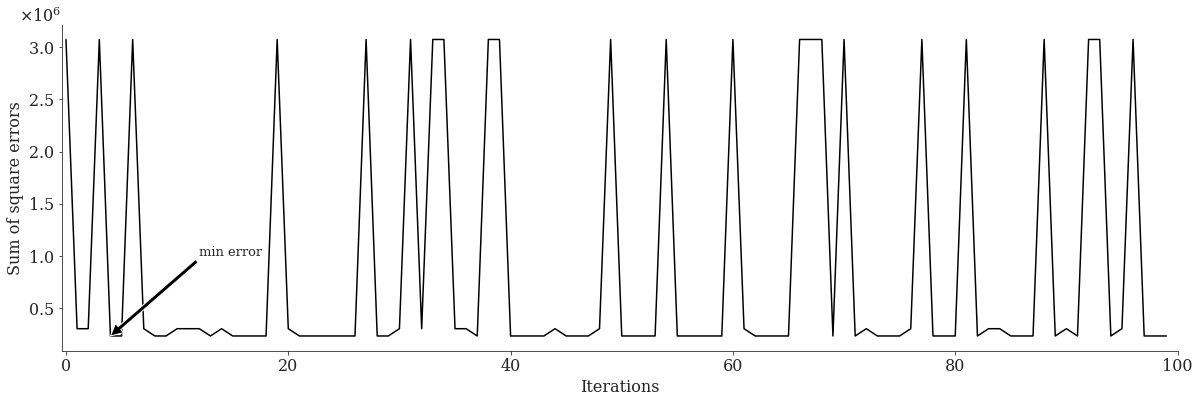
\includegraphics[width=0.8\linewidth]{./figures/ransac_error.png}
  \caption{Errors by iteration. $Y$ axis has the sum of squared differences between the target keypoints in a frame and the affine transformation of the other frame.}
  \label{fig:ransac_error}
\end{figure*}

\begin{figure*}[tb]
  \centering
  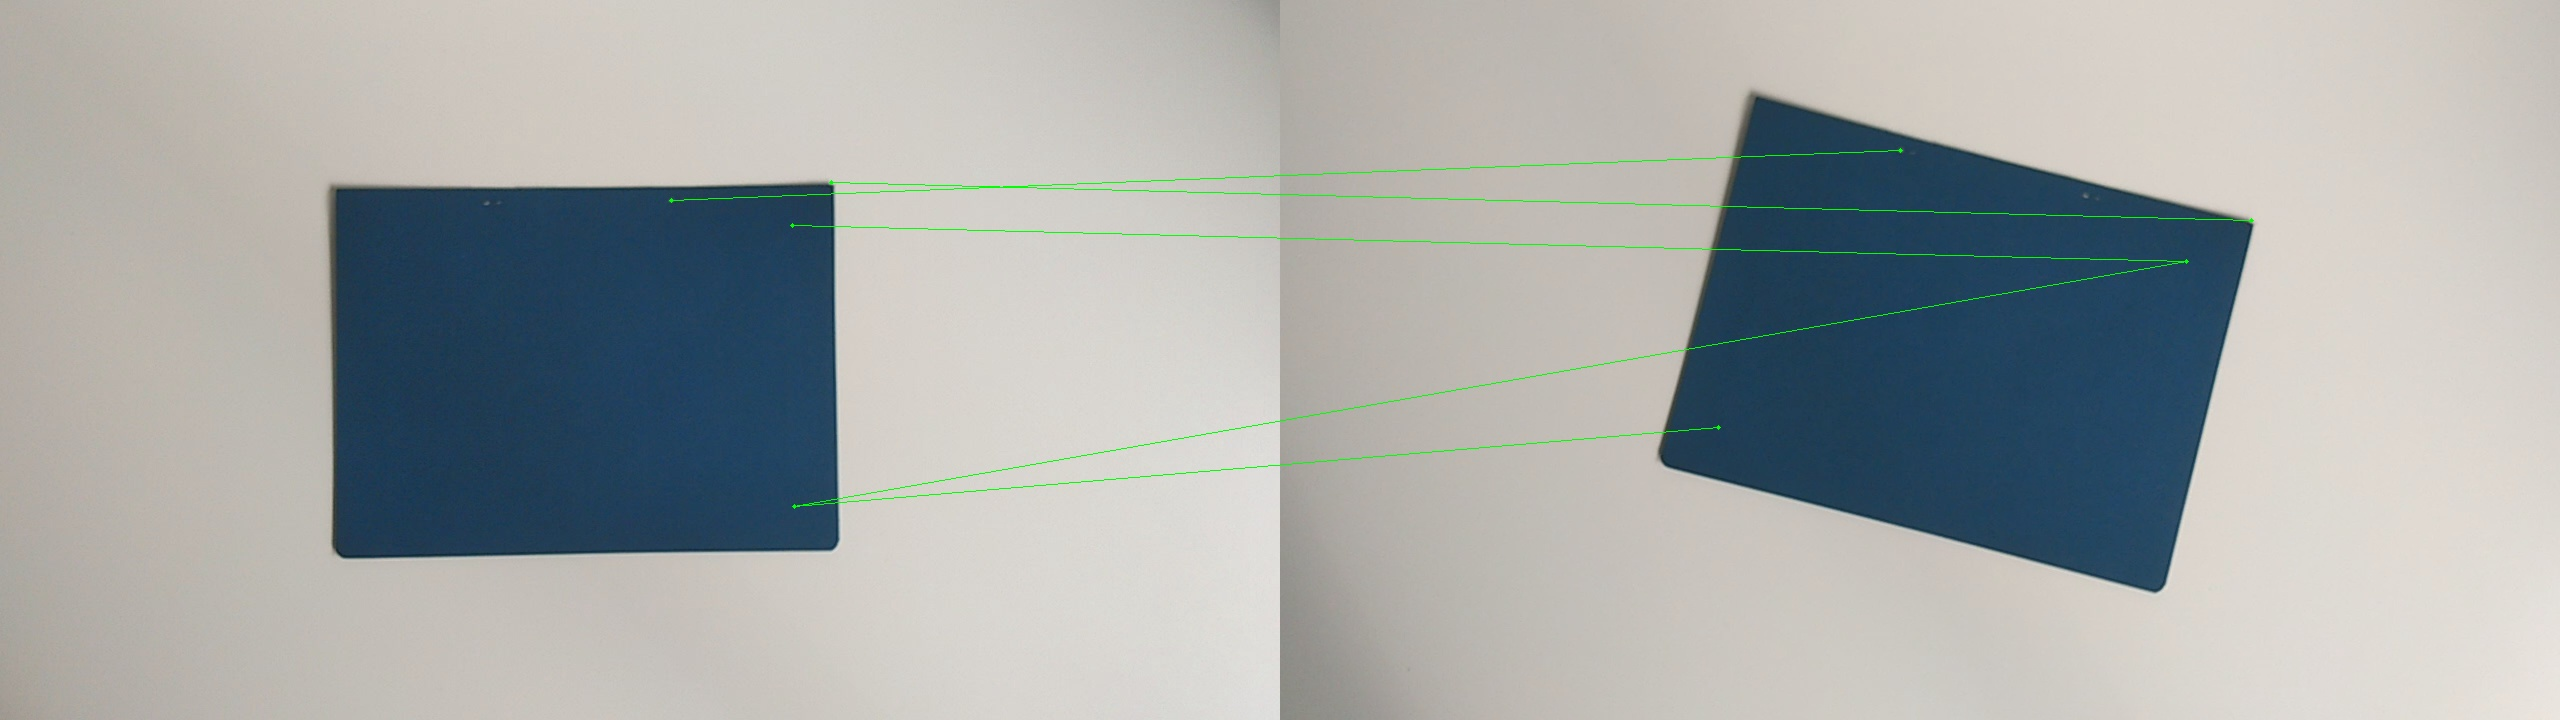
\includegraphics[width=0.8\linewidth]{./figures/feature_matching/feature_matching_1.jpg} \\
  a.~ Our $Kd$-tree matching result.\\
%   \vspace{5pt}
  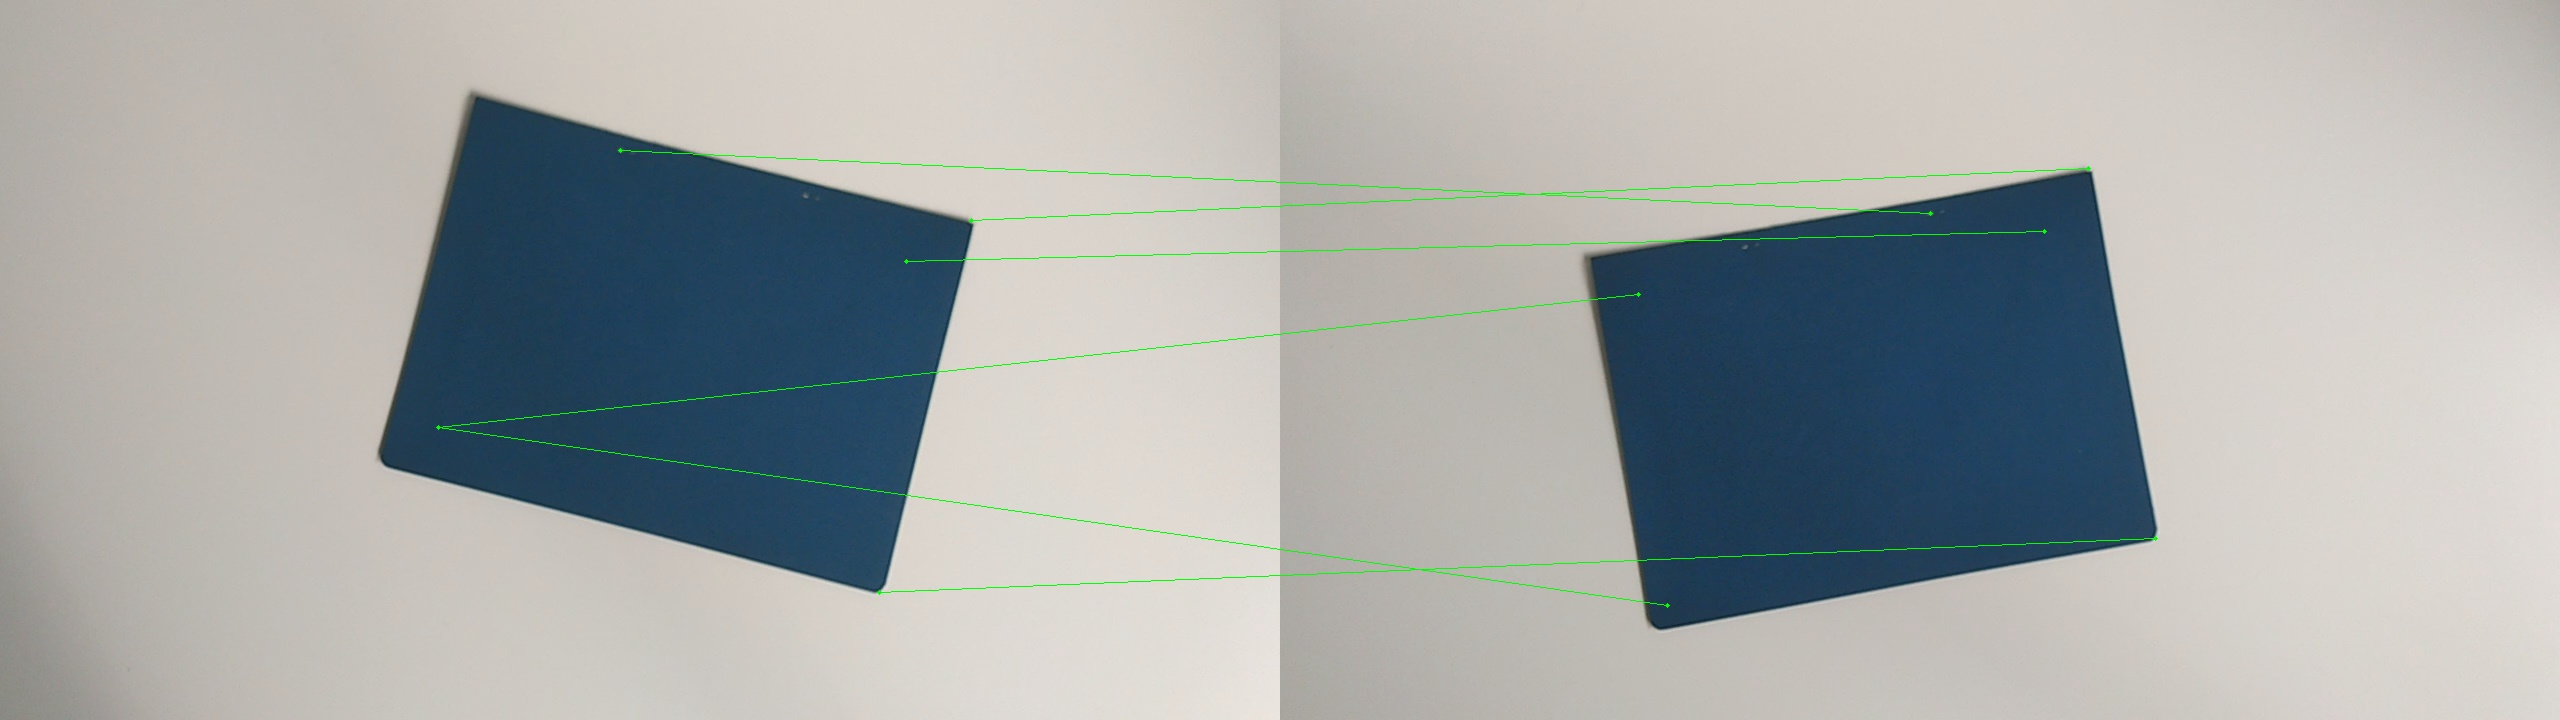
\includegraphics[width=0.8\linewidth]{./figures/feature_matching/feature_matching_2.jpg}\\
  b.~ OpenCV's FLANN $Kd$-tree matching result.
  \caption{Matching key points in four different frames}
  \label{fig:matches}
\end{figure*}

\section{Transformation}
To compute an affine transform matrix for 3 points in a 2D space, we need to solve the equation \ref{eq:3point_affine}.

% 3 points affine eq
\begin{equation} \label{eq:3point_affine}
\begin{bmatrix}
    x_1 & y_1 & 1 & 0 & 0 & 0 \\
    0 & 0 & 0 & x_1 & y_1 & 1 \\
    x_2 & y_2 & 1 & 0 & 0 & 0 \\
    0 & 0 & 0 & x_2 & y_2 & 1 \\
    x_3 & y_3 & 1 & 0 & 0 & 0 \\
    0 & 0 & 0 & x_3 & y_3 & 1 \\
\end{bmatrix}
\begin{bmatrix}
   a \\
   b \\
   c \\
   d \\
   e \\
   f \\
\end{bmatrix}
=
\begin{bmatrix}
   x_1' \\
   y_1' \\
   x_2' \\
   y_2' \\
   x_3' \\
   y_3' \\
\end{bmatrix}
\end{equation}

However, to calculate a more accurate affine transform matrix, we used more than 3 points by generalizing equation \ref{eq:3point_affine} into \ref{eq:npoint_affine}.

\begin{equation} \label{eq:npoint_affine}
\begin{bmatrix}
    x_1 & y_1 & 1 & 0 & 0 & 0 \\
    0 & 0 & 0 & x_1 & y_1 & 1 \\
    x_2 & y_2 & 1 & 0 & 0 & 0 \\
    0 & 0 & 0 & x_2 & y_2 & 1 \\
    x_i & y_i & 1 & 0 & 0 & 0 \\
    0 & 0 & 0 & x_i & y_i & 1 \\
    \dots & \dots & \dots & \dots & \dots & \dots  \\
     x_n & y_n & 1 & 0 & 0 & 0 \\
    0 & 0 & 0 & x_n & y_n & 1 \\
\end{bmatrix}
\begin{bmatrix}
   a \\
   b \\
   c \\
   d \\
   e \\
   f \\
\end{bmatrix}
=
\begin{bmatrix}
   x_1' \\
   y_1' \\
   x_2' \\
   y_2' \\
   x_i' \\
   y_i' \\
   \dots \\
   x_n' \\
   y_n' \\
\end{bmatrix}
\end{equation}

As you can see, in equation \ref{eq:npoint_affine}, each coordinate ($x_i'$, $y_i'$) is defined by a linear combination of ($x_i$, $y_i$) but restricted to the parameters ($a$, $b$, $c$, $d$, $e$, $f$). Putting in other words, we are basically learning the parameters will transform each coordinate ($x_i$, $y_i$) into ($x_i'$, $y_i'$) by providing $n$ interest points as input. You can also see that the multiplication is valid as the first matrix has dimension $2n \times 6$, the second matrix is $6 \times 1$ and the resulting matrix (with the transformed coordinates) is $2n \times 1$.

\section{Augmentation}
In this section, we'll talk about how the whole pipeline is tied together and some of the problems faced during the augmentation problem.

\subsection{Pipeline}
Our pipeline is comprised of the following steps:
\begin{enumerate}
\item Extract image frames from the input video
\item For the first frame, find the 4 corners of the rectangle and paste the target image inside it
\item For the following frames, process each consecutive pair:
\begin{enumerate}
\item Detect interest points
\item Extract features from interest points
\item Match pairs of interest points based on the feature descriptor
\item Run RANSAC to compute affine transformations with 3 points in each iteration and return the one with the highest number of inliers
\item Compute affine transformation with the inliers from the previous step
\item Transform the target image (as seen in \ref{fig:target2}) from the previous video frame
\item Paste target image on the current video frame
\end{enumerate}
\end{enumerate}

For every pair of videos frames processed, we always save the mask and the target image from the previous iteration to apply the affine transformation on them.

\subsection{Extract 4 corners}
For the first video frame, we have used a number of techniques to extract the 4 corners in the image. Although at first considered an easy task, through some attempts we realized it wasn't. An initial idea was to use DBSCAN to cluster the interest points, merge the clusters into a single point by finding the average and then considering the top 4 clusters with more points our corners. It turns out that this algorithm is very sensitive to how good or bad our interest points detector is. Even though our video scene was extremely simple (see figure \ref{fig:simple}), interest points sometimes missed one or two corners. In other cases, interest points were detected in the flat areas inside the blue rectangle or on the table surface. And in others, the matches were incorrect. Given those obstacles, we decided to approach this problem without using our interest points detector.

\begin{figure}[h]
  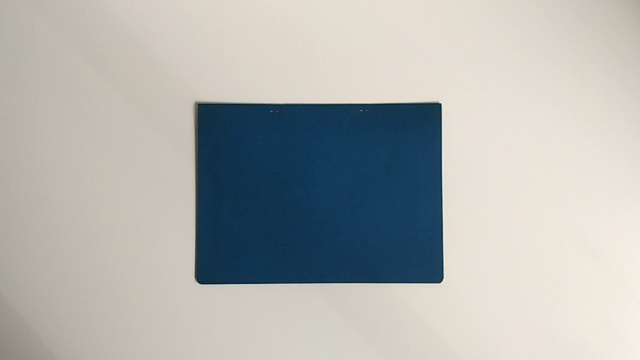
\includegraphics[width=\linewidth]{./figures/augmentation/simple.jpg}
  \caption{Video frame: a blue rectangle on a white table.}
  \label{fig:simple}
\end{figure}

Here are the steps to find the four corners:
\begin{enumerate}
    \item Apply a Gaussian filter to reduce noises
    \item Apply Canny to extract the edges of the rectangle
    \item Find continuous contours from the edges and return the one with longest perimeter
    \item Find the largest rectangle that surrounds this contour
    \item Extract the 4 coordinates of the rectangle
\end{enumerate}

Once we have the 4 coordinates of rectangle, we had to come up with some heuristic on how to determine which ones were the upper, lower, left and right corners:
\begin{enumerate}
\item First, we sort the 4 points by the x coordinate. The 2 points with the lowest x values are the left points (upper and lower left). The 2 points with the highest x values are the right points (upper and lower right).
\item Then, sort the left and the right points separately. The one with the highest y is considered the upper and the other is the lower.
\end{enumerate}

This heuristic works as long as our target frame (the blue rectangle) is not rotated in such a way that the diagonal between the lower left and the upper right points is past the 90 degrees (the vertical axis). Given that the first frame in our 3 videos had the rectangle in an horizontal position, this heuristic was sufficient to find the four corners and paste the target image into the target frame correctly.

Lastly, it's important to note that trying to fit a perfect rectangle is a limitation. Depending on the angle of the video shot, the four corners may not form a perfect rectangle and in those cases, the 4 corners found by our algorithm will not match the real corners in the image.

\subsection{Transforming the first frame}
The first frame is a special case because we don't have a previous frame to compute the transformation. Nonetheless, we created a virtual frame with the target image positioned in (0,0). We then paired the coordinates of the target image in this virtual frame with the coordinates of the 4 corners in the first frame. With these 4 pairs of coordinates, we calculated the affine transform matrix and finally applied it to the virtual frame. The result of this transformation can be seen in figures \ref{fig:target1} and \ref{fig:target2}.

\begin{figure}[h]
  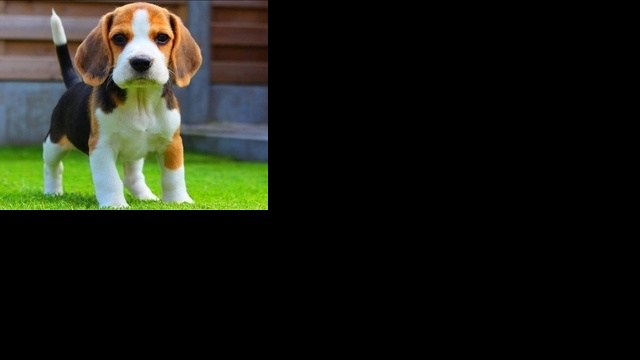
\includegraphics[width=\linewidth]{./figures/augmentation/target1.jpg}
  \caption{Target image: Virtual video frame.}
  \label{fig:target1}
\end{figure}

\begin{figure}[h]
  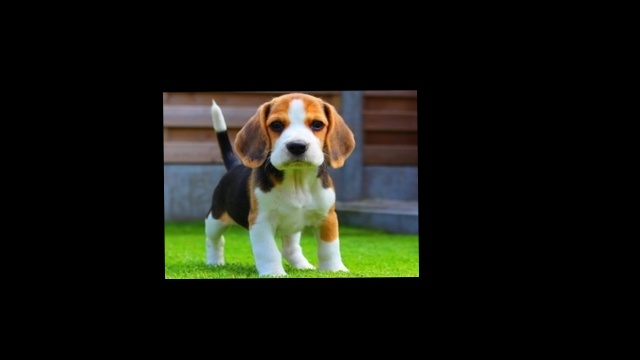
\includegraphics[width=\linewidth]{./figures/augmentation/target2.jpg}
  \caption{Target image: Virtual video frame transformed.}
  \label{fig:target2}
\end{figure}

\subsection{Resize Problem}
One of the problems that arises when we are pasting the target image into the video frame is that a transformed image may need to be padded as it won't fit perfectly the original dimension. Even a slightly rotated image already carries the problem of having zeros (black pixels) to fill in the gaps (see figure \ref{fig:affine}).

In order to solve this resize problem, we used a masking technique. At first, we create two empty images (with all zeroes) and the same dimensions as the video frame. The first one is a binary mask and it will contain only 1's in the area where the target image will be pasted on. The second will contain the target image transformed in the exact area where the binary mask has 1's. Finally, we get the original video frame (not yet processed/augmented) and we copy over only the pixel values of the target image transformed. The final result is a processed video frame as shown in Figure \ref{fig:augmentation}.

\begin{figure}[h]
  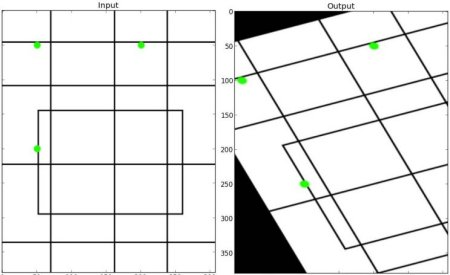
\includegraphics[width=\linewidth]{./figures/augmentation/affine.jpg}
  \caption{Affine transformation. \cite{affine_transform_image}}
  \label{fig:affine}
\end{figure}

\begin{figure}[h]
  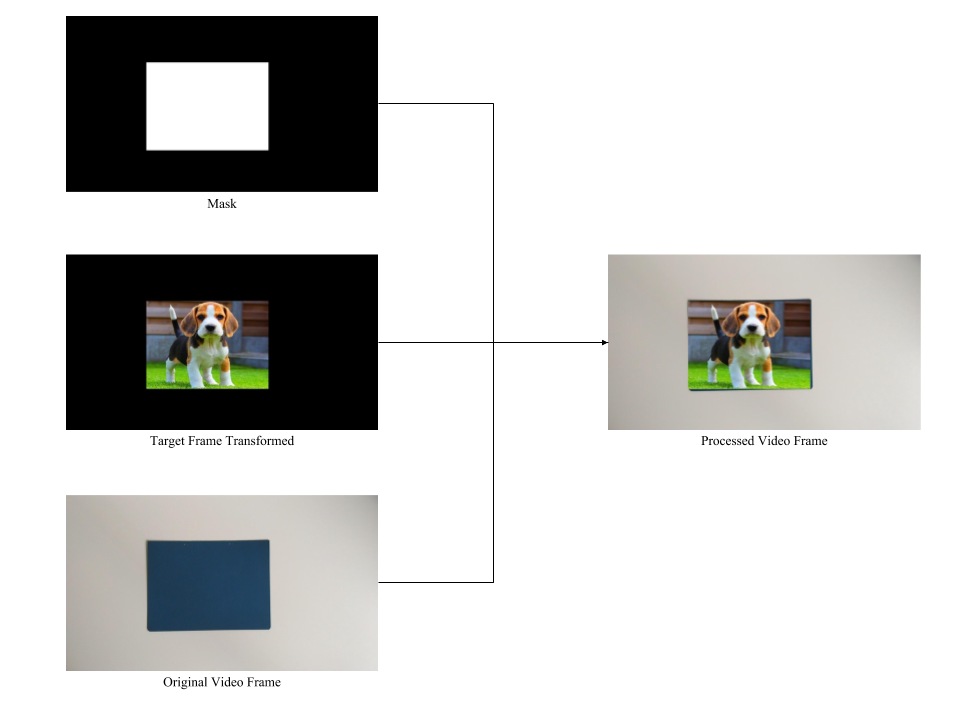
\includegraphics[width=\linewidth]{./figures/augmentation/resizing.png}
  \caption{Augmentation process.}
  \label{fig:augmentation}
\end{figure}

\section{Discussion}
\label{sec:disc}
In this section we will discuss some results, the problems observed and possible solutions. We also argue another approach to do reality augmentation resulting in a considerable improvement with respect to our pipeline. An augmented reality video produced with this method is also delivered for comparison purposes.

Our pipeline of augmented reality can be split into $7$ steps. In order to test our implementation, we ran our code on toy examples while comparing them with similar OpenCV's implementation. In most cases, our results were on par with OpenCV's. However, when we built the pipeline and ran it for all frames and videos, the final results were not as expected. Even with a pure OpenCV's implementation of the similar methods and algorithm. Later on in this section, we dive into a more technical discussion in \textit{``why''} we believe our pipeline did not behave as we expected.

\begin{figure*}[tb]
  \centering
  \begin{tabular}{c c}
  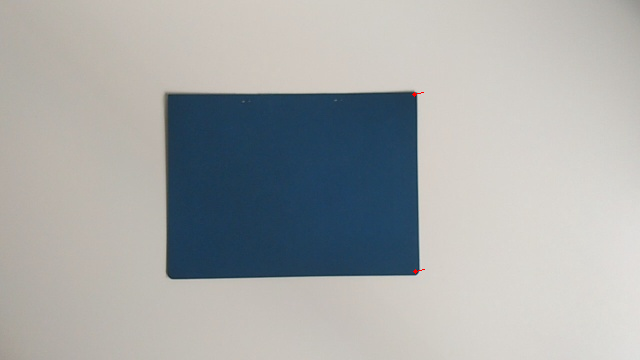
\includegraphics[width=0.48\linewidth]{./figures/sift/bad_sift.png} &
  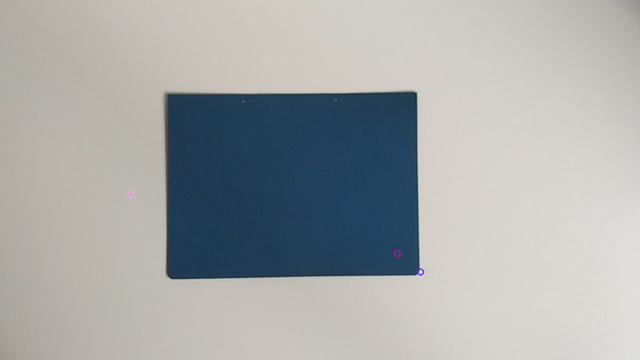
\includegraphics[width=0.48\linewidth]{./figures/sift/bad_sift_OpenCV.png}\\
  a.~Poor feature detection using our SIFT implementation & b.~Poor feature detection using OpenCV's SIFT implementation.
  \end{tabular}
  \caption{Examples of poor feature detection using SIFT.}
  \label{fig:bad_sift}
\end{figure*}

During the development of this project, we found some critical issues which certainly damaged our final results. Thus we elucidate some of these problems, discuss some causes and argue possible solutions:
\begin{itemize}
\item In most of the frames, SIFT algorithm was not able to find salient distinguishable interest points as the four corners of our target frame (the blue rectangle). Instead, it found interest points in non-salient surfaces which can be very ambiguous. Both our implementation and OpenCV's have shown poor results in several different frames of the videos as you can see in Figure \ref{fig:bad_sift}.
\item Our implementation of SIFT, made in Python, has another shortcoming that is performance. It takes about 30 seconds to detect the keypoints and compute the descriptors for a single frame, which amounts to hours when considering the full video, so we could not use our implementation as intended initially. We profiled our code using \textit{IPython} and \textit{line\_profiler} to discover that the main problem lies in a loop for every pixel of every image in the scale space. This loop computes the orientation of a keypoint in order to create its descriptor. The problem is not one particular instruction (or a set of instructions) that is running slowly, but rather the amount of times these instructions are being executed. We tried many alternative ways to perform the same operations, but none of them actually improved the execution time. The solution would be to, somehow, remove this loop altogether.
\item OpenCV's SIFT implementation has $5$ parameters to be tuned. Although we have tried to find the optimal parameters manually, we could not find one set of parameters that worked well for all frames. This same problem applies to all the pipeline steps: interest points detector, interest points feature extractor, matcher and RANSAC.
\item In several frames, our matching strategy ($Kd$-tree) and OpenCV's (FLANN $Kd$-tree) failed in delivering a good match for the set of keypoints found using SIFT. As discussed in the previous item, these poor results are not entirely due to the methods itself, but they have parameters to be tuned, and tuning them is basically impractical, once we have several frames to run the matching.
\item One bad transformation distorting the image in a frame will affect all of the following frames. This effect can be seen in some of our videos where the target image's shape rapidly degrades and then disappears. A bad transformation can be the result of bad matching of interest points, bad interest points feature extraction or bad interest points detection. All of these steps are correlated. Figure~\ref{fig:bad_match} displays an example of bad matching between two frames.
\item The fact that we are applying several affine transforms on the target image, creates a blur effect that degrades the image quality. One solution would be to apply on all frames the same 4-corners detection and transformation algorithm that we apply on the first frame.
\item The target image is not always positioned perfectly inside the target frame. After a few seconds, we can see that the distance grows between the augmented target image and the target frame. This problem is related to the first. In order to fix this, our algorithm should have some kind of recover mechanism.
\end{itemize}

\begin{figure}[h]
  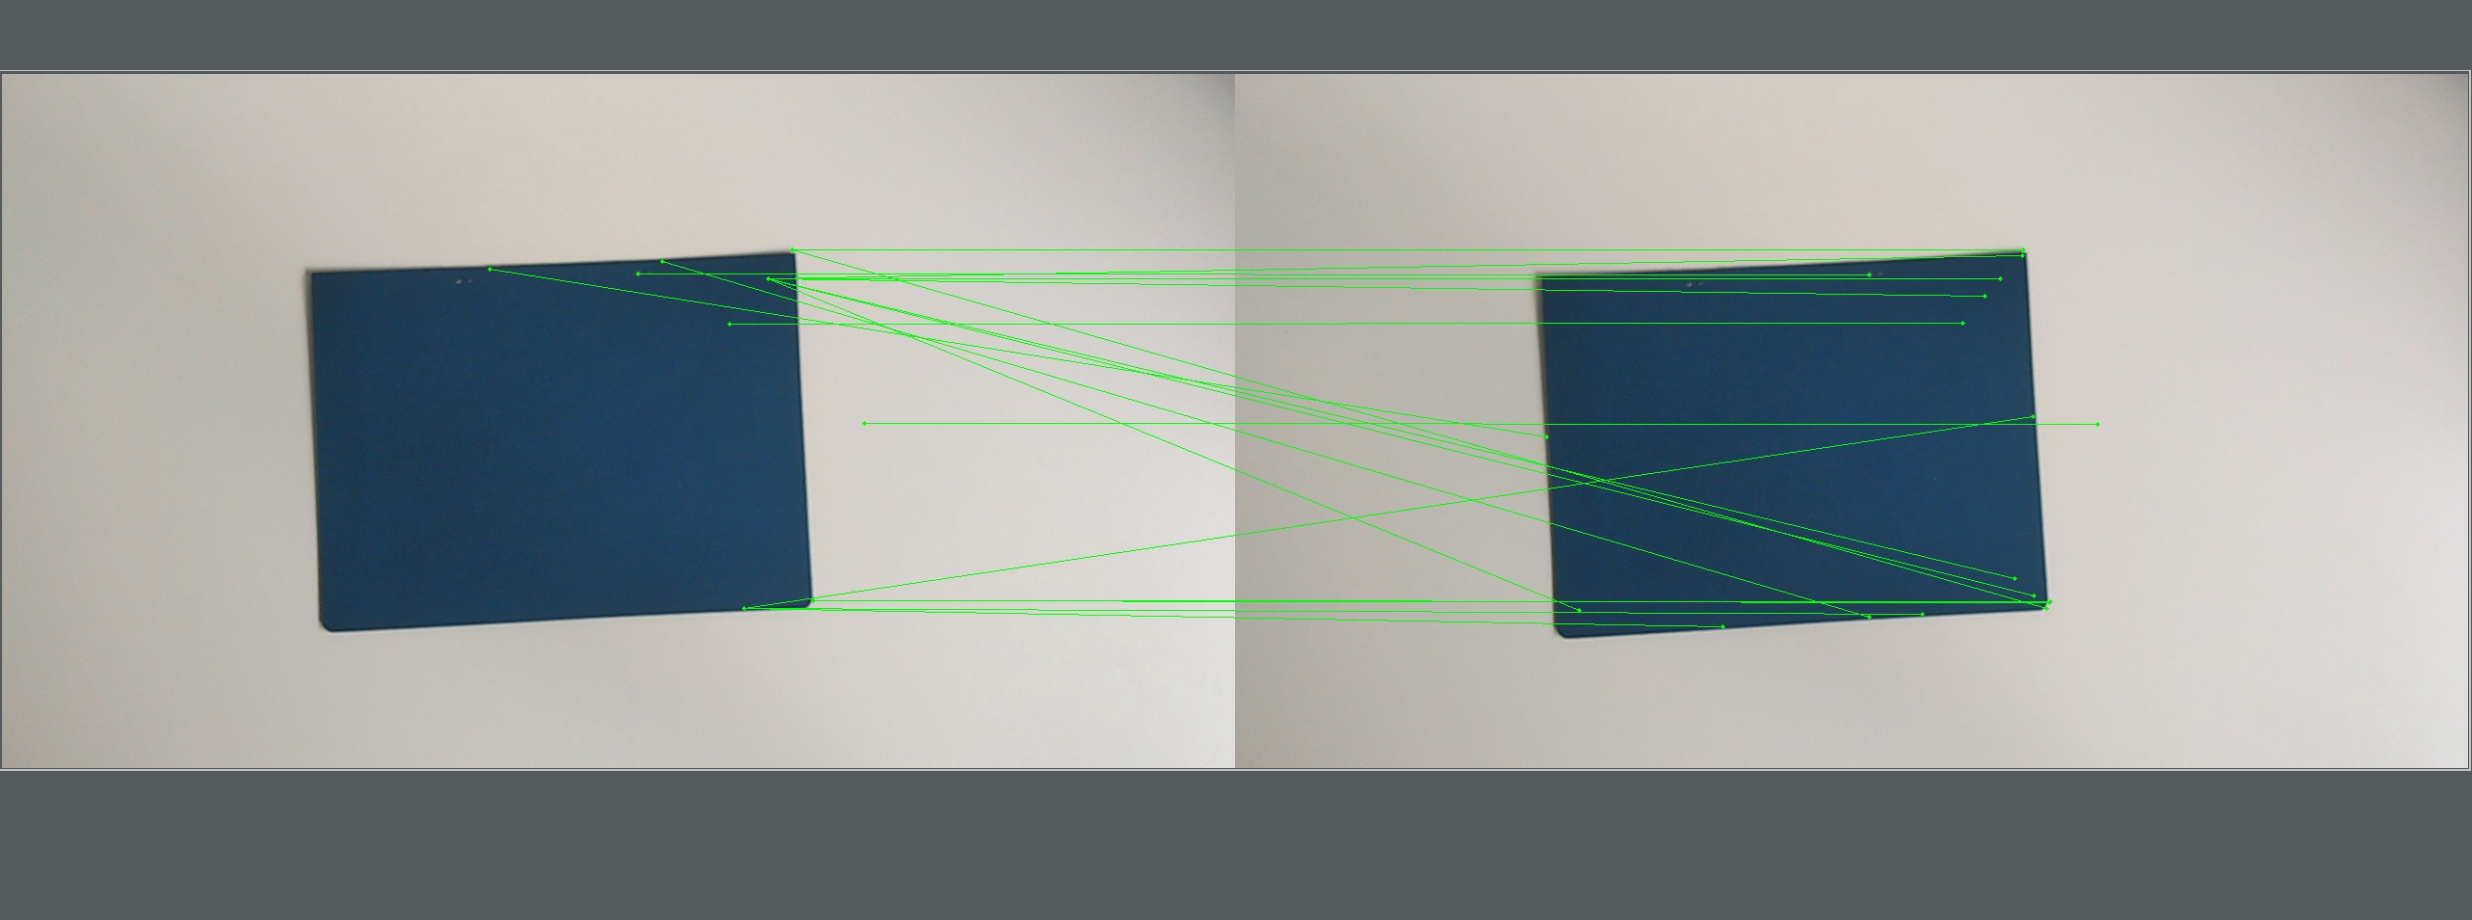
\includegraphics[width=\linewidth]{./figures/bad_match.png}
  \caption{An example of bad interest points and bad match.}
  \label{fig:bad_match}
\end{figure}

Given all of the problems above, we decided to test a pipeline replacing SIFT by the ORB keypoint detector from OpenCV. We also removed the RANSAC step and used all of the keypoints to compute the affine transformation matrix. One final difference is that we used OpenCV's matcher. We noticed that ORB's keypoints were concentrated around the 4 corners of the blue rectangle which are the only salient points in our video scene. We can also argue that the feature descriptors are less ambiguous and are more likely to generate correct matches. See Figure~\ref{fig:good_orb}. The final result is an AR (Augmented Reality) video that preserves the target image until the last frame without too much distortion. It's also clear in this video the relationship between the camera motion and the target image transformation.

\begin{figure}[h]
  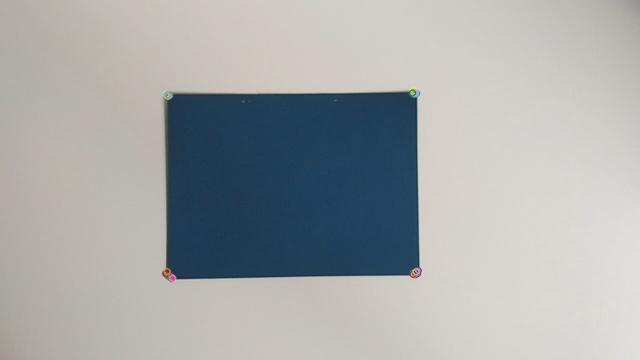
\includegraphics[width=\linewidth]{./figures/good_orb.png}
  \caption{ORB: An example of good interest points.}
  \label{fig:good_orb}
\end{figure}

\section{Conclusion}
In this work, we revisited a simple augmented reality task which was placing an image inside another image. In our case, we placed an image inside a set of images representing a video. Our pipeline is divided in $7$ building blocks: detection of interest points (keypoints); feature extraction; feature matching; using RANSAC to find $3$ keypoints with the smallest quadratic error; evaluation of the affine transformation with these $3$ points from last step; using the affine matrix to project an image in a target frame and then joining the images to produce the video.

We discuss each of the aforementioned blocks in previous sections. In Section \ref{sec:disc}, we discuss some of our results and problems found during the development of this project. Given that we faced a number of problems, two pipeline versions are delivered. The first one was implemented as defined in the project requirements with the exception of the SIFT algorithm (we used OpenCV's). The results were far from successful and did not produce the AR effect expected. In the very early frames, the affine transformation distorts the target image several time causing it to quickly disappear from the video. The second version used OpenCV's ORB, OpenCV's matcher and no RANSAC. The final result was substantially better when compared to the first pipeline. We can clearly see the AR effect and the target image is much more stable throughout the video.

As our SIFT implementation was too slow to run to process our 3 videos, we resorted to OpenCV's SIFT implementation. Nevertheless, our SIFT code has been committed to GitLab and we provide 10 frame examples of interest points found in the artifacts files.

\begin{thebibliography}{00}
    \bibitem{iccv99} Lowe, D. G. (1999, September). Object Recognition from Local Scale-Invariant Features. In Proc. of the International Conference on Computer Vision.
    \bibitem{ijcv04} Lowe, D. G. (2004, January). Distinctive Image Features from Scale-Invariant Keypoints. In International Journal of Computer Vision, 2004.
    \bibitem{sift_kdtree} Li, M., Wang, L., \& Hao, Y. (2010, April). Image matching based on SIFT features and kd-tree. In Computer Engineering and Technology (ICCET), 2010 2nd International Conference on (Vol. 4, pp. V4-218). IEEE.
    \bibitem{kd_tree} Bentley, J. L. (1975). Multidimensional binary search trees used for associative searching. Communications of the ACM, 18(9), 509-517.
    \bibitem{comp_geo} Berg, M. D., Cheong, O., Kreveld, M. V., \& Overmars, M. (2008). Computational geometry: algorithms and applications. Springer-Verlag TELOS.
    \bibitem{moore_penrose} Ben-Israel, A., \& Greville, T. N. (2003). Generalized inverses: theory and applications (Vol. 15). Springer Science \& Business Media.
    \bibitem{ransac} Fischler, M. A., \& Bolles, R. C. (1981). Random sample consensus: a paradigm for model fitting with applications to image analysis and automated cartography. Communications of the ACM, 24(6), 381-395.
    \bibitem{moore_pen_site} The Moore Penrose Pseudoinverse [Web blog post]. Retrieved
        September 21, 2018, from
        https://hadrienj.github.io/posts/Deep-Learning-Book-Series-2.9-The-Moore-Penrose-Pseudoinverse/
    \bibitem{flann} Muja, M., \& Lowe, D. G. (2009). Fast approximate nearest neighbors with automatic algorithm configuration. VISAPP (1), 2(331-340), 2.
    \bibitem{wikipedia_kd2d} k-d tree [Wikipedia page]. Retrieved
        September 21, 2018, from
        https://upload.wikimedia.org/wikipedia/commons/b/bf/Kdtree\_2d.svg
    \bibitem{wikipedia_kd1d} k-d tree [Wikipedia page]. Retrieved
        September 21, 2018, from
        https://en.wikipedia.org/wiki/K-d\_tree\#/media/File:Tree\_0001.svg
    \bibitem{affine_transform_image} Image retrieved on September 21, 2018, from \url{https://docs.opencv.org/3.0-beta/doc/py_tutorials/py_imgproc/py_geometric_transformations/py_geometric_transformations.html}
\end{thebibliography}
\end{document}
